\documentclass[10pt]{article}

\usepackage{spheric}
%%%TITLE
\title{Numerical simulation of green water using SPH method}
\date{}

%%AFFILIATIONS
\author[$\relax$]{Liang-Jun WEN}
\author[$\relax$]{Qiang-dong FENG}
\affil[$\relax$]{China Ship Scientific Research Center, Wuxi 214082,China}

%\affil[$\relax$]{\email{\dagger}{}}


%%DOCUMENT
\begin{document}

\maketitle

%\SelectedTopics{}

%%PLEASE PUT YOUR ABSTRACT HERE
\begin{abstract}
When the ship is navigating in the sea, it is inevitable to meet the rough sea condition. In this case, the ship can suffer great danger from green water, and severe green water can cause structure damages. The flows tend to be highly dynamic, with large amounts of free surface deformation. A numerical method to simulate the phenomenon of the green water on deck is established by taking advantage of SPH method.

The paper aims to extend this method to deal with green water. The ship motion is given by potential flow theory. The ship model is regard as rigid body. Numerical results of water flow on deck and green water loads on the deck structure are compared with the corresponding experimental data. It is shown that the SPH method can be applied to describe and analyze green water.

\begin{figure}[!htb]
\begin{minipage}[b]{0.44\linewidth}
\centering
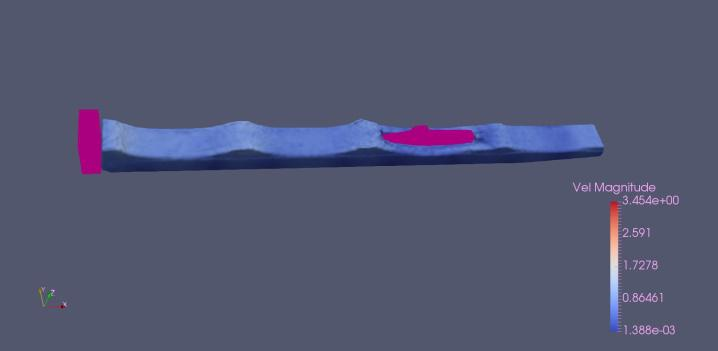
\includegraphics[width=\textwidth]{32-11.png}
\end{minipage}
\begin{minipage}[b]{0.05\linewidth}
~
\end{minipage}
\begin{minipage}[b]{0.48\linewidth}
\centering
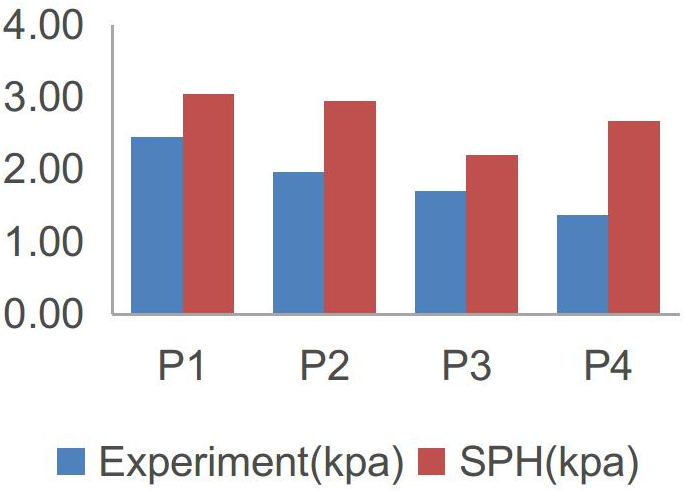
\includegraphics[width=0.8\textwidth]{32-12.png}
\end{minipage}
\end{figure}

\end{abstract}


%%THE END OF ABSTRACT

\addbib

\end{document}
